 \documentclass[journal,12pt,twocolumn]{IEEEtran}
%
\usepackage{setspace}
\usepackage{gensymb}
%\doublespacing
\singlespacing

%\usepackage{graphicx}
%\usepackage{amssymb}
%\usepackage{relsize}
\usepackage[cmex10]{amsmath}
%\usepackage{amsthm}
%\interdisplaylinepenalty=2500
%\savesymbol{iint}
%\usepackage{txfonts}
%\restoresymbol{TXF}{iint}
%\usepackage{wasysym}
\usepackage{amsthm}
%\usepackage{iithtlc}
\usepackage{mathrsfs}
\usepackage{txfonts}
\usepackage{stfloats}
\usepackage{bm}
\usepackage{cite}
\usepackage{cases}
\usepackage{subfig}
%\usepackage{xtab}
\usepackage{longtable}
\usepackage{multirow}
%\usepackage{algorithm}
%\usepackage{algpseudocode}
\usepackage{enumitem}
\usepackage{mathtools}
\usepackage{steinmetz}
\usepackage{tikz}
\usepackage{circuitikz}
\usepackage{verbatim}
\usepackage{tfrupee}
\usepackage[breaklinks=true]{hyperref}
%\usepackage{stmaryrd}
\usepackage{tkz-euclide} % loads  TikZ and tkz-base
%\usetkzobj{all}
\usetikzlibrary{calc,math}
\usepackage{listings}
    \usepackage{color}                                            %%
    \usepackage{array}                                            %%
    \usepackage{longtable}                                        %%
    \usepackage{calc}                                             %%
    \usepackage{multirow}                                         %%
    \usepackage{hhline}                                           %%
    \usepackage{ifthen}                                           %%
  %optionally (for landscape tables embedded in another document): %%
    \usepackage{lscape}     
\usepackage{multicol}
\usepackage{chngcntr}
%\usepackage{enumerate}

%\usepackage{wasysym}
%\newcounter{MYtempeqncnt}
\DeclareMathOperator*{\Res}{Res}
%\renewcommand{\baselinestretch}{2}
\renewcommand\thesection{\arabic{section}}
\renewcommand\thesubsection{\thesection.\arabic{subsection}}
\renewcommand\thesubsubsection{\thesubsection.\arabic{subsubsection}}

\renewcommand\thesectiondis{\arabic{section}}
\renewcommand\thesubsectiondis{\thesectiondis.\arabic{subsection}}
\renewcommand\thesubsubsectiondis{\thesubsectiondis.\arabic{subsubsection}}

% correct bad hyphenation here
\hyphenation{op-tical net-works semi-conduc-tor}
\def\inputGnumericTable{}                                 %%

\lstset{
%language=C,
frame=single, 
breaklines=true,
columns=fullflexible
}
%\lstset{
%language=tex,
%frame=single, 
%breaklines=true
%}

\begin{document}
%
\newtheorem{theorem}{Theorem}[section]
\newtheorem{problem}{Problem}
\newtheorem{proposition}{Proposition}[section]
\newtheorem{lemma}{Lemma}[section]
\newtheorem{corollary}[theorem]{Corollary}
\newtheorem{example}{Example}[section]
\newtheorem{definition}[problem]{Definition}
%\newtheorem{thm}{Theorem}[section] 
%\newtheorem{defn}[thm]{Definition}
%\newtheorem{algorithm}{Algorithm}[section]
%\newtheorem{cor}{Corollary}
\newcommand{\BEQA}{\begin{eqnarray}}
\newcommand{\EEQA}{\end{eqnarray}}
\newcommand{\define}{\stackrel{\triangle}{=}}
\bibliographystyle{IEEEtran}
%\bibliographystyle{ieeetr}
\providecommand{\mbf}{\mathbf}
\providecommand{\pr}[1]{\ensuremath{\Pr\left(#1\right)}}
\providecommand{\qfunc}[1]{\ensuremath{Q\left(#1\right)}}
\providecommand{\sbrak}[1]{\ensuremath{{}\left[#1\right]}}
\providecommand{\lsbrak}[1]{\ensuremath{{}\left[#1\right.}}
\providecommand{\rsbrak}[1]{\ensuremath{{}\left.#1\right]}}
\providecommand{\brak}[1]{\ensuremath{\left(#1\right)}}
\providecommand{\lbrak}[1]{\ensuremath{\left(#1\right.}}
\providecommand{\rbrak}[1]{\ensuremath{\left.#1\right)}}
\providecommand{\cbrak}[1]{\ensuremath{\left\{#1\right\}}}
\providecommand{\lcbrak}[1]{\ensuremath{\left\{#1\right.}}
\providecommand{\rcbrak}[1]{\ensuremath{\left.#1\right\}}}
\theoremstyle{remark}
\newtheorem{rem}{Remark}
\newcommand{\sgn}{\mathop{\mathrm{sgn}}}
\providecommand{\abs}[1]{\left\vert#1\right\vert}
\providecommand{\res}[1]{\Res\displaylimits_{#1}} 
\providecommand{\norm}[1]{\left\lVert#1\right\rVert}
%\providecommand{\norm}[1]{\lVert#1\rVert}
\providecommand{\mtx}[1]{\mathbf{#1}}
\providecommand{\mean}[1]{E\left[ #1 \right]}
\providecommand{\fourier}{\overset{\mathcal{F}}{ \rightleftharpoons}}
%\providecommand{\hilbert}{\overset{\mathcal{H}}{ \rightleftharpoons}}
\providecommand{\system}{\overset{\mathcal{H}}{ \longleftrightarrow}}
	%\newcommand{\solution}[2]{\textbf{Solution:}{#1}}
\newcommand{\solution}{\noindent \textbf{Solution: }}
\newcommand{\cosec}{\,\text{cosec}\,}
\providecommand{\dec}[2]{\ensuremath{\overset{#1}{\underset{#2}{\gtrless}}}}
\newcommand{\myvec}[1]{\ensuremath{\begin{pmatrix}#1\end{pmatrix}}}
\newcommand{\mydet}[1]{\ensuremath{\begin{vmatrix}#1\end{vmatrix}}}
\newcommand\inv[1]{#1\raisebox{1.15ex}{$\scriptscriptstyle-\!1$}}

%\numberwithin{equation}{section}
\numberwithin{equation}{subsection}
%\numberwithin{problem}{section}
%\numberwithin{definition}{section}
\makeatletter
\@addtoreset{figure}{problem}
\makeatother
\let\StandardTheFigure\thefigure
\let\vec\mathbf
%\renewcommand{\thefigure}{\theproblem.\arabic{figure}}
\renewcommand{\thefigure}{\theproblem}
%\setlist[enumerate,1]{before=\renewcommand\theequation{\theenumi.\arabic{equation}}
%\counterwithin{equation}{enumi}
%\renewcommand{\theequation}{\arabic{subsection}.\arabic{equation}}
\def\putbox#1#2#3{\makebox[0in][l]{\makebox[#1][l]{}\raisebox{\baselineskip}[0in][0in]{\raisebox{#2}[0in][0in]{#3}}}}
     \def\rightbox#1{\makebox[0in][r]{#1}}
     \def\centbox#1{\makebox[0in]{#1}}
     \def\topbox#1{\raisebox{-\baselineskip}[0in][0in]{#1}}
     \def\midbox#1{\raisebox{-0.5\baselineskip}[0in][0in]{#1}}
\vspace{3cm}
\title{EE5609: Matrix Theory\\
          Assignment-5\\}
\author{M Pavan Manesh\\
EE20MTECH14017 }
\maketitle
\newpage
%\tableofcontents
\bigskip
\renewcommand{\thefigure}{\theenumi}
\renewcommand{\thetable}{\theenumi}
\begin{abstract}
This document contains solution to determine the conic representing the given equation. 
\end{abstract}
Download the python codes from 
%
%
latex-tikz codes from 
%
\begin{lstlisting}
https://github.com/pavanmanesh/EE5609/tree/master/Assignment5
\end{lstlisting}
%
\section{Problem}
What conic does the following equation represent. 
\begin{align*}
9x^2-24xy+16y^2-18x-101y+19 = 0
\end{align*}
Find the center.
\section{Solution}
The general second degree equation can be expressed as follows,
\begin{align}
\vec{x^T}\vec{V}\vec{x}+2\vec{u^T}\vec{x}+f=0\label{eqmain}
\end{align}
From the given second degree equation we get,
\begin{align}
\vec{V} &= \myvec{9&-12\\-12&16}\\ \label{given1}
\vec{u} &= \myvec{-9\\-\frac{101}{2}}\\ 
f &= 4 \label{given2}
\end{align}
Expanding the determinant of $\vec{V}$ we observe, 
\begin{align}
\mydet{9&-12\\-12&16} = 0 \label{eq2.1}
\end{align}
Also
\begin{align}
    \mydet{\vec{V} & \vec{u} \\ \vec{u}^T & f}=
    \mydet{9&-12 & -9 \\-12&16 & -\frac{101}{2} \\ -9 & -\frac{101}{2} & 4} \\
    \neq 0\label{eq2.2}
\end{align}
Hence from \eqref{eq2.1} and \eqref{eq2.2} we conclude that given equation is an parabola. The characteristic equation of $\vec{V}$ is given as follows,
\begin{align}
\mydet{\lambda\vec{I}-\vec{V}} = \mydet{\lambda-9&12\\12&\lambda-16} &= 0\\
\implies \lambda^2-25\lambda &= 0\label{eqchar}
\end{align}
Hence the characteristic equation of $\vec{V}$ is given by \eqref{eqchar}. The roots of \eqref{eqchar} i.e the eigenvalues are given by
\begin{align}
\lambda_1=0, \lambda_2=25\label{eqeigenvals}    
\end{align}
The eigen vector $\vec{p}$ is defined as, 
\begin{align}
\vec{V}\vec{p} &= \lambda\vec{p}\\
\implies\brak{\lambda\vec{I}-\vec{V}}\vec{p}&=0 \label{eqev}
\end{align}
for $\lambda_1=0$,
\begin{align}
\brak{\lambda_1\vec{I}-\vec{V}}&=\myvec{-9&12\\12&-16}\xleftrightarrow[R_1=\frac{1}{-9}R_1]{R_2=3R_1-R_2}\myvec{1&-\frac{4}{3}\\0&0}\\
\implies\vec{p_1}&=\myvec{\frac{1}{\sqrt{3}}\\1} \label{eq2.3}
\end{align}
Substiuting equation \ref{eq2.3} in equation \ref{eqev} we get
\begin{align}
&\myvec{1&-\frac{4}{3}\\0&0}\myvec{v_1 \\ v_2}=\myvec{0 \\ 0}\label{eqei1}
\end{align}
Where, $\vec{p}=\myvec{v_1\\v_2}$
Let $v_2=t$
\begin{align}
    v_1&=\frac{4}{3}t
\end{align}
Eigen vector $\vec{p_1}$ is given by
\begin{align}
    \vec{p_1}&=\myvec{\frac{4}{3}t \\ t}
\end{align}
Let $t=-\frac{6}{10}$, we get
\begin{align}
        \vec{p_1}&=\myvec{-\frac{8}{10} \\-\frac{6}{10} }\label{eqp1}
\end{align}
Again, for $\lambda_2=25$,
\begin{align}
\brak{\lambda_2\vec{I}-\vec{V}}&=\myvec{16&12\\12&9}\xleftrightarrow[R_1=\frac{1}{16}R_1]{R_2=12R_1-R_2}\myvec{1&\frac{3}{4}\\0&0} \label{eq2.3.1}
\end{align}
Substiuting equation \ref{eq2.3.1} in equation \ref{eqev} we get
\begin{align}
&\myvec{1&\frac{3}{4}\\0&0}\myvec{v_1 \\ v_2}=\myvec{0 \\ 0}\label{eqei1}
\end{align}
Where, $\vec{p}=\myvec{v_1\\v_2}$
Let $v_2=t$
\begin{align}
    v_1&=-\frac{3}{4}t
\end{align}
Eigen vector $\vec{p_2}$ is given by
\begin{align}
    \vec{p_2}&=\myvec{-\frac{3}{4}t \\ t}
\end{align}
Let $t=-\frac{8}{10}$, we get
\begin{align}
        \vec{p_2}&=\myvec{\frac{6}{10} \\-\frac{8}{10} }\label{eqp1}
\end{align}
The matrix \vec{P},
\begin{align}
\vec{P}&=\myvec{\vec{p_1}&\vec{p_2}}=\myvec{-\frac{8}{10}&\frac{6}{10}\\-\frac{6}{10}&-\frac{8}{10}} \\
\vec{D}&=\myvec{0&0\\0&25}
\end{align}
\begin{align}
    \eta=2\vec{u}^T\vec{p_1}=75
\end{align}
The focal length of the parabola is given by:
\begin{align}
    \abs{\frac{\eta}{\lambda_2}} 
    = \frac{75}{25}=3
\end{align}
When $\mydet{\vec{V}}=0$,\eqref{eqmain} can be written as
\begin{align}
    \vec{y^T}\vec{D}\vec{y}&=-\eta\myvec{1&0}\vec{y}\label{eq2.4}
    \intertext{And the vertex $\vec{c}$ is given by }
    \myvec{\vec{u^T}+\eta\vec{p_1^T} \\ \vec{V}}\vec{c}=
    \myvec{-f \\ \eta\vec{p_1}-\vec{u}} 
\end{align}
using equations \eqref{given1},\eqref{given2} and \eqref{eq2.3}
\begin{align}
    \myvec{-69& -\frac{191}{2} \\ 9 & -12 \\  -12 & 16 }\vec{c}=\myvec{-4 \\ -51 \\ \frac{11}{2}} \label{eqcen}
\end{align}
 This is in the form of 
 \begin{align}
 {A}\vec{c}=\vec{b}
 \end{align}
  \begin{align} 
 \intertext{using least squares solution of linear system}
 {A}^T{A}\vec{c}={A}^T\vec{b}
 \implies \vec{c}=  ({{A}^T{A}})^{-1} {A}^T\vec{b} \label{main}
\end{align}
\begin{align}
{A}^T{A}=\myvec{-69 & 9 & -12 \\ -\frac{191}{2}& -12& 16 }
 \myvec{-69& -\frac{191}{2} \\ 9 & -12 \\  -12 & 16 } \nonumber \\ \implies
 {A}^T{A}=\myvec{4986& \frac{12579}{2} \\  \frac{12579}{2} & \frac{38081}{4} }
\end{align}
The inverse can be written as
\begin{align}
    ({{A}^T{A}})^{-1}=\frac{31640625}{4}
    \myvec{\frac{38081}{4}&- \frac{12579}{2} \\  -\frac{12579}{2} & 4986}\label{con1}
\end{align} 
\begin{align}
   {A}^T\vec{b} = \myvec{-69 & 9 & -12 \\ -\frac{191}{2}& -12& 16 }\myvec{-4 \\ -51 \\ \frac{11}{2}} \nonumber \\
   {A}^T\vec{b} =\myvec{-249 \\ 1082} \label{con2}
\end{align}
using \ref{con1} and \ref{con2} in \ref{main},the center $\vec{c}$
\begin{align}
    \vec{c}=\frac{31640625}{4}
    \myvec{\frac{38081}{4}&- \frac{12579}{2} \\  -\frac{12579}{2} & 4986}\myvec{-249 \\ 1082} \\
    \implies \vec{c}=\myvec{-\frac{29}{25} \\ \frac{22}{25}} 
\end{align}

\renewcommand{\thefigure}{1}
\begin{figure}[!ht]
    \centering
    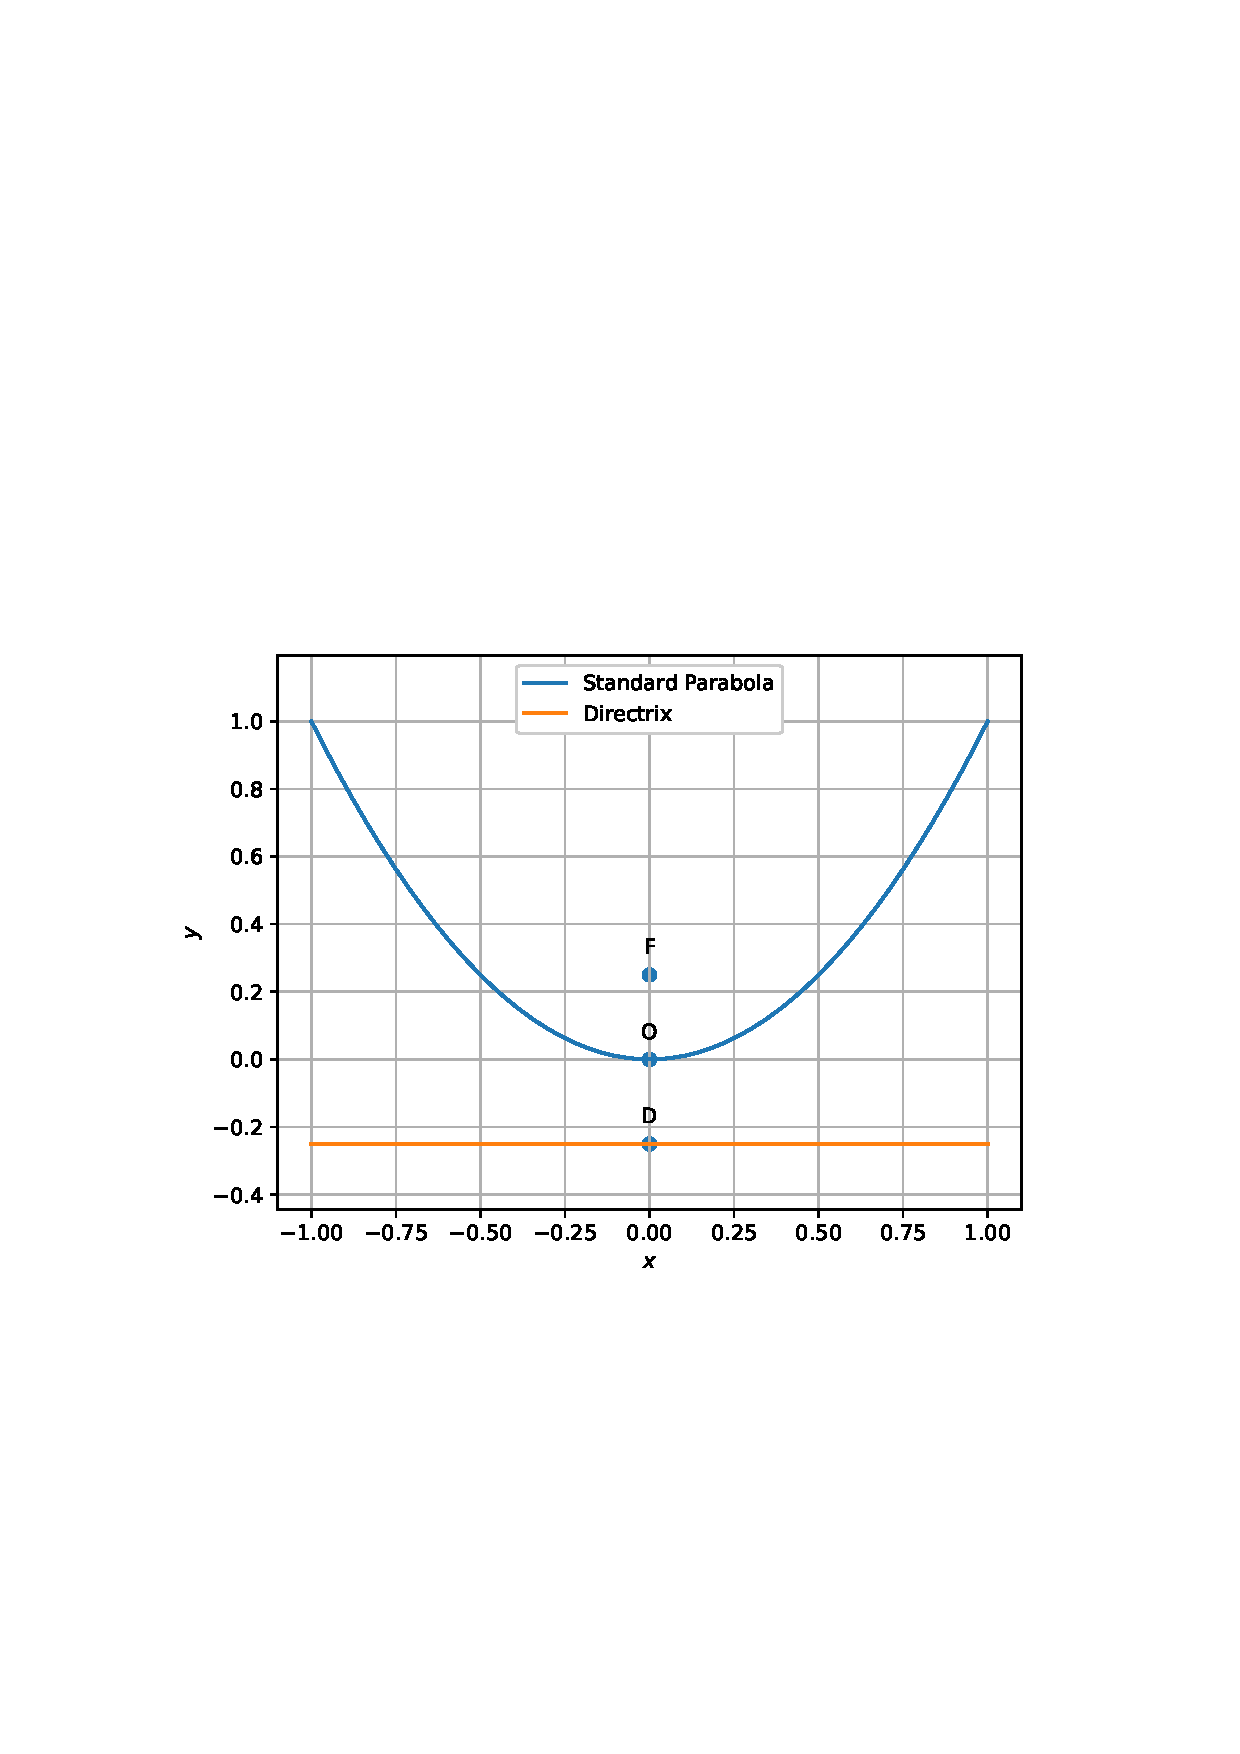
\includegraphics[width=\columnwidth]{parabola.png}
    \caption{Parabola with the center c}
    \label{Fig:1}
\end{figure}
\end{document}
